\section{Vektorgeometrie}

\subsection{Gerade}
\noindent Parameterdarstellung: \[\vec{p} = \vec{p}_0 + t\vec{r} \left\lbrace 
	\begin{array}{r@{\quad}l}
		\vec{p}_0 & \text{Stützvektor}\\ 
		\vec{r}  & \text{Richtungsvektor} \\
		t & \text{Streckfaktor}
	\end{array}
\right. \]


\subsection{Ebene}
\noindent Parameterdarstellung: \[\vec{p} = \vec{p}_0 +  t\vec{u} + s\vec{v} \left\lbrace 
\begin{array}{r@{\quad}l}
	\vec{p}_0 & \text{Stützvektor} \\ 
	\vec{u},\vec{v}  & \text{Richtungsvektor} \\
	t,s & \text{Streckfaktor}
\end{array}
\right. \]

\noindent Normalform: \label{normalform}
\[
	\vec{n} \circ \vec{PQ} = \vec{n} \circ (\vec{q} - \vec{p}) = 0
\]
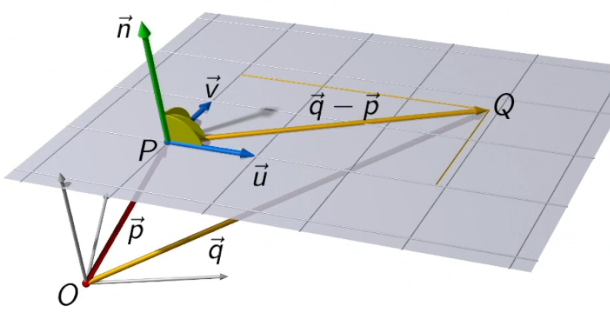
\includegraphics[width=\columnwidth]{./Images/Normalenform.png}
\[
	n_1x + n_2y + n_3z = n_4 \left\lbrace 
	\begin{array}{r@{\quad}l}
		n_4 & \text{Länge der Normale: } \vec{n} \circ \vec{p} \\ 
		n_{1-3} & \text{Normale } \vec{n} = \begin{pmatrix}n_1\\n_2\\n_3\end{pmatrix}
	\end{array}
	\right.
\]

\subsection{Kreis und Kugel}
\noindent Vektorgleichung:
\[(\vec{p} - \vec{m})^2 = r^2\]

\noindent Koordinatengleichung:
\[ (x - m_x)^2 + (y - m_y)^2 = r^2 \left\lbrace \begin{array}{r@{\quad}l}
		$m$ & \text{ist Mittelpunkt des Kreises}\\
		$r$ & \text{ist Radius}
	\end{array}\right.
\]
\noindent In dieser Form können Radius und Mittelpunkt abgelesen werden. Beispiel:
\[x^2 - 4x +y^2 + 6y - 12 = 0\]
Quadratische Ergänzung um Mittelpunkt $m = (2, -3)$ und Radius $r = 5$ zu erhalten:
\begin{align*}
	(x^2 - 4x + \textcolor{red}{2^2}) &+ (y^2 + 6y + \textcolor{red}{3^2}) \textcolor{blue}{- 2^2 - 3^2} - 12 &= 0 \\
	(x - 2)^2 &+ (y + 3)^2 &= 5^2
\end{align*}

\subsubsection{Durchstosspunkt}
Geradengleichung $\vec{p} = \vec{p}_0 + \textcolor{red}{s} \cdot \vec{r}$ in Kugelgleichung einsetzen:
\[
	(\vec{p}_0 + \textcolor{red}{s} \cdot \vec{r} - \vec{m}) \circ (\vec{p}_0 + \textcolor{red}{s} \cdot \vec{r} - \vec{m}) = r^2
\]

\[
	\vec{r} \circ \vec{r}  \cdot \textcolor{red}{s^2} + 2(\vec{p}_0 - \vec{m}) \circ \vec{r} \cdot \textcolor{red}{s} + (\vec{p}_0 - \vec{m})\circ(\vec{p}_0 - \vec{m}) - r^2  =0
\]

\begin{center}
	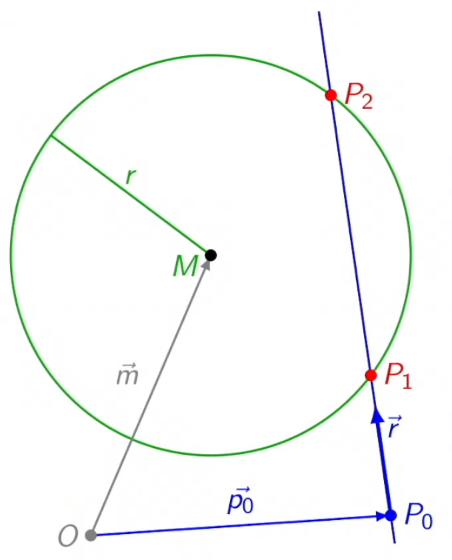
\includegraphics[width=12em]{./Images/Kugelgleichung.png}
\end{center}

\noindent Anschliessend Quadratische Gleichung nach $\textcolor{red}{s}$ auflösen um Durchstosspunkte zu erhalten.

\subsection{Schnittmenge}
Die Schnittmenge kann in $\mathbb{R}^n$ mit der Schnittmengenmatrix und Gauss bestimmt werden. \\
Beispiel:
\[
	\left.
	\begin{aligned}
		\text{Ebene } \sigma_1 : \textcolor{red}{\vec{p}} &= \vec{p}_1 + \textcolor{red}{t_1} \vec{u}_1 + \textcolor{red}{s_1} \vec{v}_1 \\
		\text{Ebene } \sigma_2 : \textcolor{red}{\vec{p}} &= \vec{p}_2 + \textcolor{red}{t_2} \vec{u}_2 + \textcolor{red}{s_2} \vec{v}_2 \\
	\end{aligned}
	\right\rbrace
	\Rightarrow
	\text{Gerade } g: \textcolor{red}{\vec{p}} = \vec{q} + \textcolor{green}{s_2} \vec{r}
\]

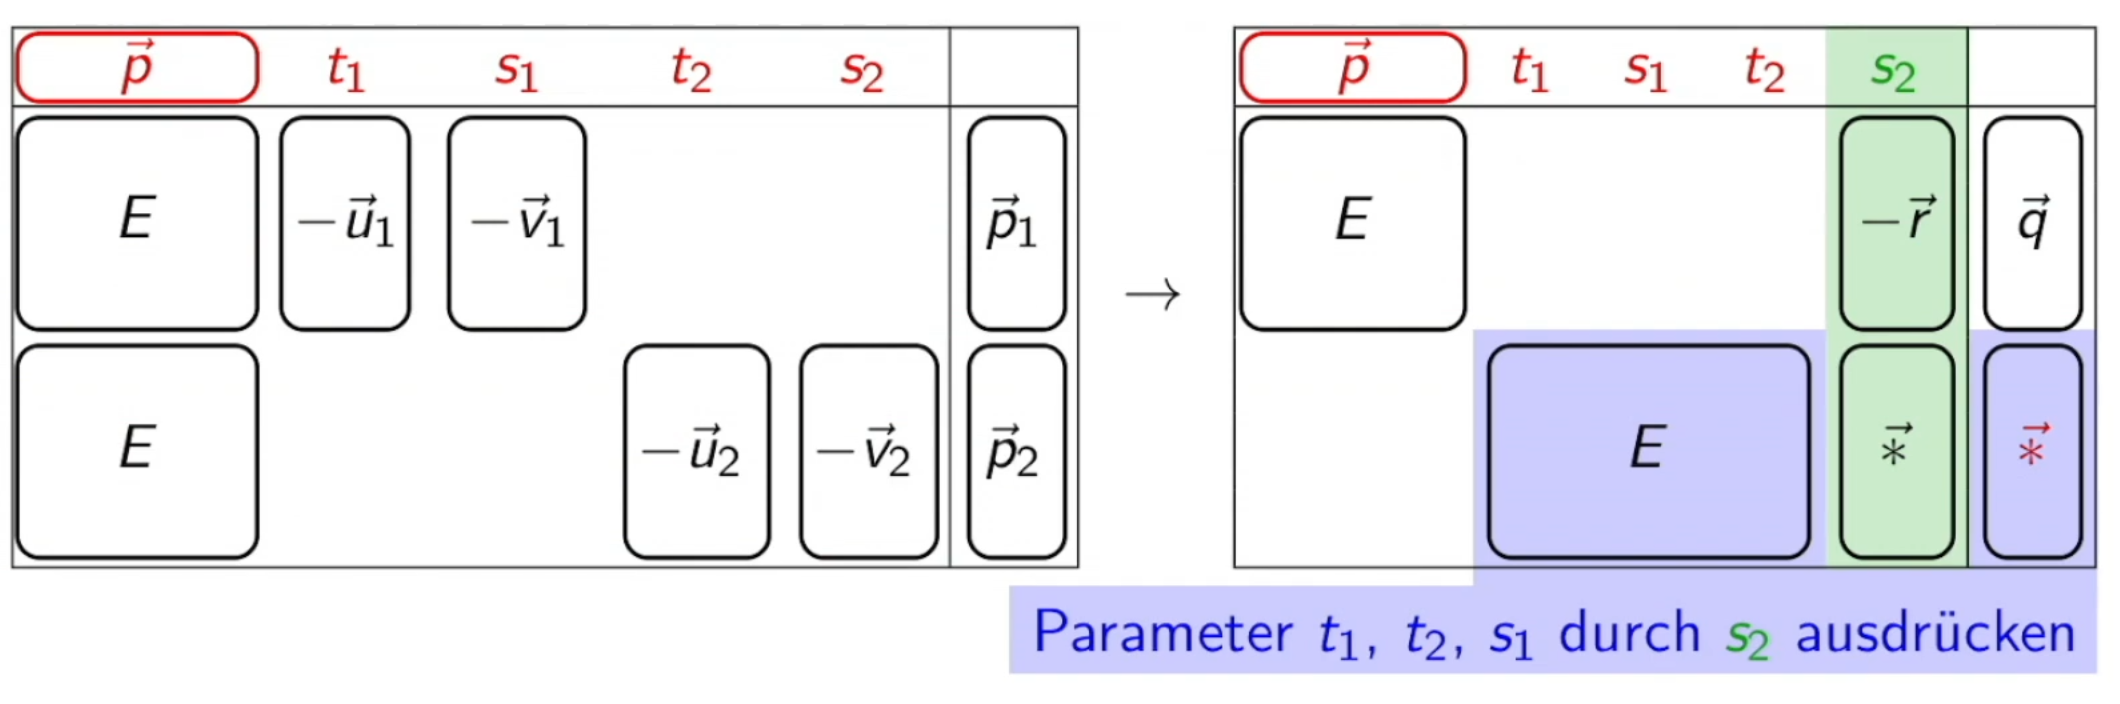
\includegraphics[width=\columnwidth]{./Images/Schnittmenge.png}

\subsection{Skalarprodukt}
\[\vec{a} \circ \vec{b} = \begin{pmatrix} x_a \\ y_a \\ z_a \end{pmatrix} \circ \begin{pmatrix} x_b \\ y_b \\ z_b \end{pmatrix} = x_a \cdot x_b + y_a \cdot y_b + z_a \cdot z_b\]

Eigenschaften:
\begin{itemize}[nosep]
	\item Länge: $\vec{a} \circ \vec{a} =|\vec{a}|^2$
	\item Spezial-Fall Rechtwinklig: $ \vec{a} \perp \vec{b} \Rightarrow \vec{a} \circ \vec{b} = 0 $
	\item Matrix Schreibweise: $\vec{a} \circ \vec{b} \eqi \vec{a}^T\cdot\vec{b} = \vec{a}\cdot\vec{b}^T$
\end{itemize}

\subsubsection{Zwischenwinkel}
\[\cos{\alpha} = \frac{\vec{a} \circ \vec{b}}{|\vec{a}| \cdot |\vec{b}|}\]

\subsubsection{Orthogonale Projektion}
Die orthogonale Projektion eines Vektors auf einen anderen entspricht der Streckung oder Stauchung eines Vektors und zwar in der Art, dass der \textit{Schatten} des projizierten Vektors orthogonal auf ihm steht.

\begin{center}
	\begin{minipage}{0.20\textwidth}
		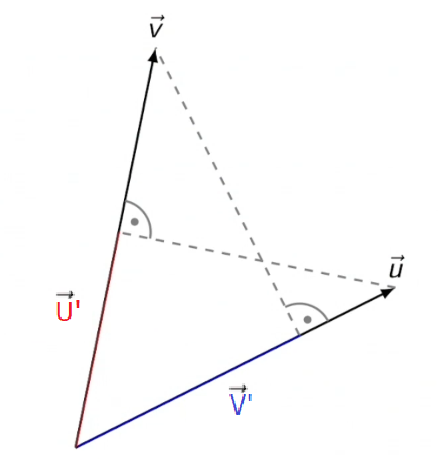
\includegraphics[width=\linewidth,keepaspectratio=true]{./Images/skalarprojektion.png}
	\end{minipage}%%% to prevent a space
	\begin{minipage}{0.2\textwidth}
		\[\vec{v}' = \frac{\vec{v} \circ \vec{u}}{\left|\vec{u}\right|^2} \cdot \vec{u}\]
		\[\vec{u}' = \frac{\vec{u} \circ \vec{v}}{\left|\vec{v}\right|^2} \cdot \vec{v}\]
	\end{minipage}
\end{center}

\subsection{Vektorprodukt}
Das \textbf{Vektorprodukt} steht senkrecht auf beiden Vektoren ($\vec{a}, \vec{b}$) und hat die Länge der Grundfläche.

\begin{center}	
	\tikzset{ x=1mm, y=1mm }
	\begin{tikzpicture}
		\node {$\vec{a} \times \vec{b} = \begin{pmatrix}
				-2 & 10 \\
				3 & 2 \\
				1 & -1 \\
				-2 & 10 \\
				3 & 2 \\
				1 & -1 \\
			\end{pmatrix} = \begin{pmatrix}
				(\textcolor{blue}{3 \cdot (-1)}) - (\textcolor{red}{1 \cdot 2}) \\
				(\textcolor{blue}{1 \cdot 10}) - (\textcolor{red}{(-2) \cdot (-1)}) \\
				(\textcolor{blue}{(-2) \cdot 2}) - (\textcolor{red}{10 \cdot 3}) \\
			\end{pmatrix} = \begin{pmatrix}
				-5 \\
				8 \\
				-34 \\
			\end{pmatrix}$
		};
		\draw[line width=0.2mm,gray, dashed] (-34,0) -- (-16, 0);
		
		\draw[line width=0.4mm,blue] (-27,6) -- (-23,3);
		\draw[line width=0.4mm,blue] (-27,2) -- (-23,-1);
		\draw[line width=0.4mm,blue] (-27,-2) -- (-23,-5);
		
		\draw[line width=0.4mm,red] (-27,3) -- (-23,6);
		\draw[line width=0.4mm,red] (-27,-1) -- (-23,2);
		\draw[line width=0.4mm,red] (-27,-5) -- (-23,-2);
		
		\draw[line width=0.2mm,black] (-34,11) -- (-16,11);
		\draw[line width=0.2mm,black] (-34,-10) -- (-16,-10);	
	\end{tikzpicture}	
\end{center}

\subsubsection{Zwischenwinkel}
Auch beim Vektorprodukt ergibt sich ein Zwischenwinkel:
\[\sin\alpha = \frac{\left|\vec{a}_0 \times \vec{a}_1\right|}{\left|\vec{a}_0\right| \cdot \left|\vec{a}_1\right|}\]

\subsection{Spur}\label{drehwinkel}
Die Spur ist die Summe der Diagonal-Elemente. In $\mathbb{R}^3$ gilt daher (Spur ist in allen Achsen gleich):
\[
	D_z = \begin{pmatrix}
		\cos(\alpha) & -\sin(\alpha) & 0 \\
		\sin(\alpha) & \cos(\alpha) & 0 \\
		0 & 0 & 1
	\end{pmatrix} \rightarrow  Spur(D_\alpha) = 2 \cdot \cos(\alpha) + 1 
\]
\noindent Daraus ergibt sich die allgemeine Formel für $\mathbb{R}^3$: \\$\cos(\alpha) = \frac{Spur(D_\alpha) - 1}{2}$. \\\textbf{Achtung} in $\mathbb{R}^2$ ist es $\cos(\alpha) = \frac{Spur(D_\alpha)}{2}$

\subsection{Spiegelung}
Um eine Abbildung zu Spiegeln, muss ein Normalvektor $\vec{n}$ zur Spiegelachse existieren werden.

\begin{center}
	\begin{minipage}{0.25\textwidth}
		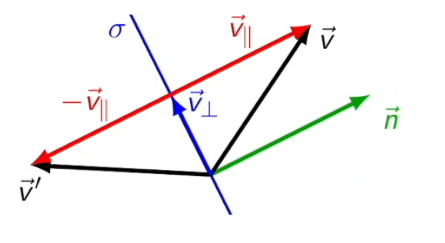
\includegraphics[width=\linewidth,keepaspectratio=true]{./Images/Spiegelung.png}
	\end{minipage}%%% to prevent a space
	\begin{minipage}{0.2\textwidth}
		Vektor Spiegelung:
		\[\vec{v}' = \vec{v} - 2\vec{n}\frac{\vec{n} \circ \vec{v}}{|\vec{n}|^2}\]

		Matrix Spiegelung:
		\[S = E - 2\frac{1}{|\vec{n}|^2}\vec{n}\vec{n}^T\]
	\end{minipage}
\end{center}

\subsection{Abstand}
\noindent Abstand zwischen Punkt $Q$ und Gerade $\vec{p} = \vec{p}_0 + t\vec{r}$: 
\begin{center}
	\begin{minipage}{0.25\textwidth}
		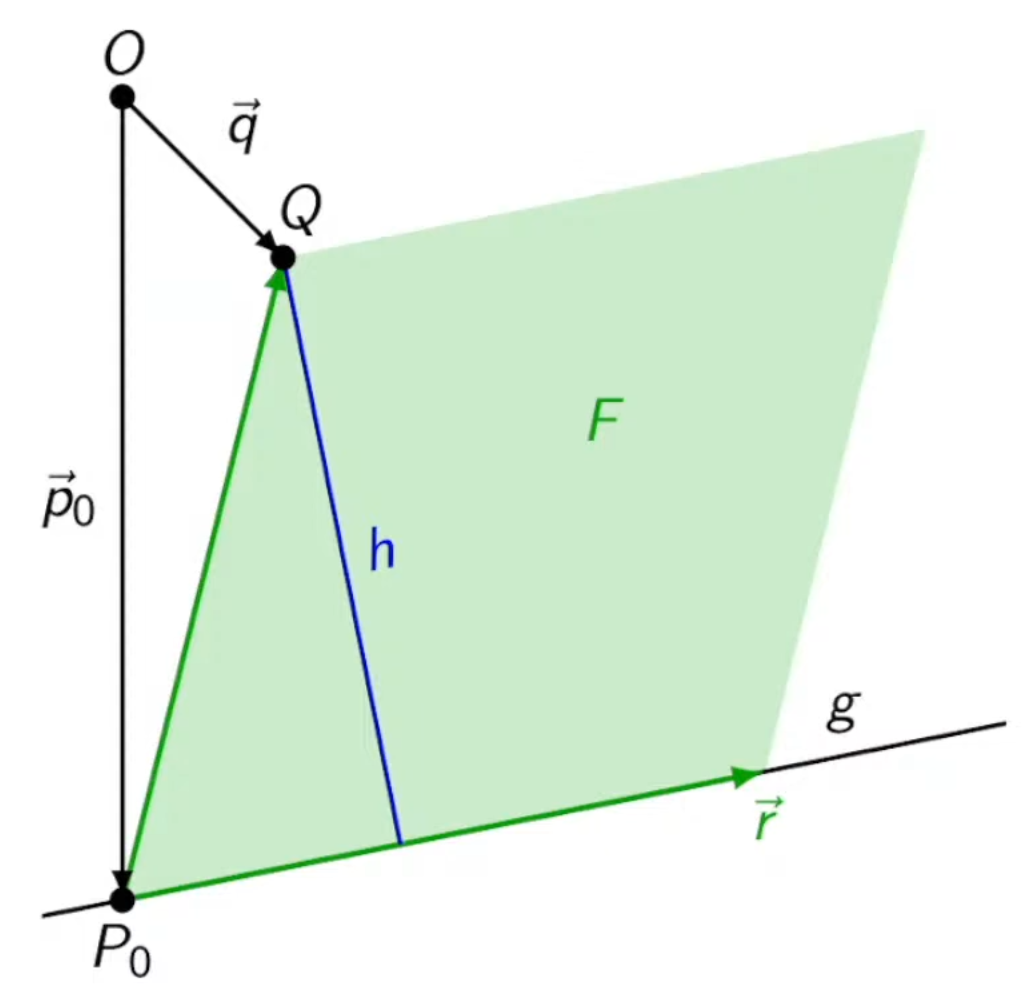
\includegraphics[width=\linewidth,keepaspectratio=true]{./Images/AbstandPunkt.png}
	\end{minipage}%%% to prevent a space
	\begin{minipage}{0.2\textwidth}
			$h = \frac{\left|\vec{r} \times (\vec{q} - \vec{p}_1)\right|}{\left|\vec{r}\right|}$
	\end{minipage}
\end{center}

\noindent Abstand zwischen zwei Geraden $\vec{p} = \vec{p}_1 + t\vec{r}_1$ und $\vec{p}' = \vec{p}_2 + s\vec{r}_2$:
\begin{center}
	\begin{minipage}{0.25\textwidth}
		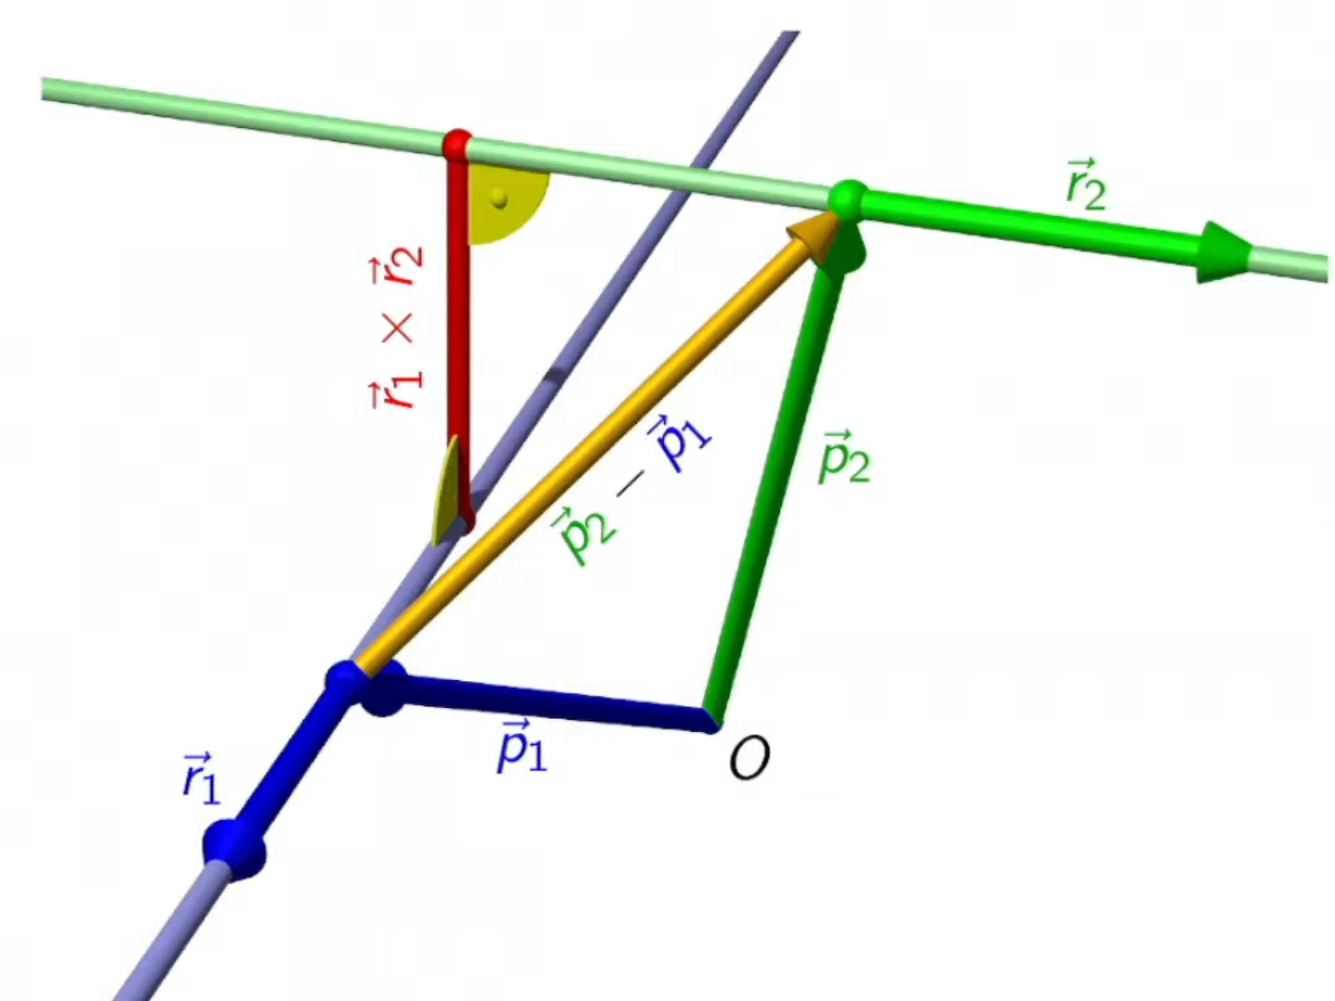
\includegraphics[width=\linewidth,keepaspectratio=true]{./Images/AbstandGerade.png}
	\end{minipage}%%% to prevent a space
	\begin{minipage}{0.2\textwidth}
		$h = (\vec{p}_2 - \vec{p}_1) \circ \frac{\vec{r}_1 \times \vec{r}_2}{|\vec{r}_1 \times \vec{r}_2|}$
	\end{minipage}
\end{center}


\noindent Allgemein:
$h = \frac{V_{n+1}}{v_n} = \sqrt{\frac{Gram(b, a_1, \dots, a_k)}{Gram(a_1, \dots, a_k)}}$

\subsubsection{Hes'sche Normalform}
Dient häufig zur Berechnung von Abständen von Punkten nach Geraden ($\mathbb{R}^2$) oder Ebenen ($\mathbb{R}^3$).

\[
d = \frac{(\vec{q} - \vec{p}) \circ \vec{n}}{|\vec{n}|} = \frac{n_1}{|\vec{n}|}x + \frac{n_2}{|\vec{n}|}y + \frac{n_3}{|\vec{n}|}z - \frac{\vec{n} \circ \vec{p}}{|\vec{n}|}
\] 

\noindent Siehe auch \verweiseref{normalform} Normalform.\\

\noindent Beispiel: \\
Hes'sche Normalform finden, indem $\vec{n}$ mit Richtungsvektoren $\vec{r}_1$ und $\vec{r}_2$ von der Ebenengleichung orthogonal sind.
\[
\underbrace{\begin{pmatrix}1 \\ 2 \\ 1 \end{pmatrix}}_{\vec{p}} + \underbrace{t \begin{pmatrix}2 \\ 2 \\ -2 \end{pmatrix}}_{\vec{r}_1} + \underbrace{s \begin{pmatrix}3 \\ -3 \\ -1 \end{pmatrix}}_{\vec{r}_2}
\]

\begin{align*}
	\vec{n} \circ \vec{r}_1 = 0 \quad &\Rightarrow \quad 2n_1 + 2n_2 - 3n_3 = 0 \\
	\vec{n} \circ \vec{r}_2 = 0 \quad &\Rightarrow \quad 3n_1 - 3n_2 - n_3 = 0
\end{align*}

\[
\begin{array}{|ccc|c|}
	\hline
	2 & 2 & -2 & 0 \\
	3 & -3 & -1 & 0 \\
	\hline
\end{array} \xrightarrow{Gauss}
\begin{array}{|ccc|c|}
	\hline
	1 & 0 & -\frac{2}{3} & 0 \\
	0 & 1 & -\frac{1}{3} & 0 \\
	\hline
\end{array} 
\]

\noindent Die Normale ist $\vec{n} = \begin{pmatrix} 2 \\ 1 \\ 3 \end{pmatrix}$. 
Diese muss nun noch auf die Länge $1$ gestutzt werden und in die korrekte Form gebracht werden.  Durch einsetzen eines beliebigen Punktes kann der Abstand $d$ von der entsprechenden Ebene berechnet werden.
\[
\underbrace{\frac{\vec{n}}{\left|\vec{n}\right|}}_{\text{Normiert } \vec{n}^0}  \circ \left(\begin{pmatrix} x \\ y \\ z \end{pmatrix} - \underbrace{\begin{pmatrix} 1 \\ 2 \\ 1 \end{pmatrix}}_{\vec{p}} \right) = d
\]


\subsection{Schuhbändelformel}
Mit der Schuhbändelformel kann ein Flächeninhalt eines Polygons ($P1 \dots Pn$) in $\mathbb{R}^2$ berechnet werden. \textcolor{orange}{\textbf{Achtung:}} Erster Punkt muss am Schluss nochmals gerechnet werden! ($P_1 = P_n$)

\begin{center}
	$F = \frac{1}{2}\sum\limits_{n = 1}^{k}(\textcolor{blue}{P_{n}x \cdot P_{n+1}y } - \textcolor{red}{P_{n}y \cdot P_{n+1}x })$
	
	\tikzset{ x=1mm, y=1mm }
	\begin{tikzpicture}
		\node {$F = \frac{1}{2}\begin{vmatrix}
				P_1x & P_1y \\
				P_2x & P_2y \\
				P_3x & P_3y \\
				P_4x & P_4y \\
				\vdots & \vdots \\
				\textcolor{orange}{P_1x} & \textcolor{orange}{P_1y} \\
			\end{vmatrix}$
		};
		\draw[line width=0.4mm,blue] (4,11) -- (7,8);
		\draw[line width=0.4mm,blue] (4,7) -- (7,4);
		\draw[line width=0.4mm,blue] (4,3) -- (7,0);
		\draw[line width=0.4mm,blue] (4,-1) -- (7,-4);
		
		\draw[line width=0.4mm,red] (4,8) -- (7,11);
		\draw[line width=0.4mm,red] (4,4) -- (7,7);
		\draw[line width=0.4mm,red] (4,0) -- (7,3);
		\draw[line width=0.4mm,red] (4,-4) -- (7,-1);
	\end{tikzpicture}	
\end{center}

\noindent
Um eine Dreickes-Fläche $ABC$ in $\mathbb{R}^3$ zu berechnen kann folgende Formel verwendet werden:
\[F = \frac{\left|\vec{AB} \times \vec{AC}\right|}{2}\]

\noindent
Mit der Gram-Determinante kann auch eine Fläche berechnet werden \verweiseref{gram-determinante}.

\subsection{Orthogonalisieren}\label{orthogonalisieren}
Sucht Vektoren im gegeben Raum ($\mathbb{R}^n$) und stellt diese Orthogonal (rechtwinklig) zu einander. 
\\ \\
\textbf{Beispiel}
Lineare unabhängige Vektoren $\{\vec{a}_1, ..., \vec{a}_n\}$ $\rightarrow$ orthonormierte Vektoren $\{\vec{b}_1, ..., \vec{b}_n\}$
\begin{align*}
	\vec{b}_1 &= \vec{a}_1 \\
	\vec{b}_2 &= \vec{a}_2 - \frac{\vec{a}_2 \circ \vec{b}_1}{|\vec{b}_1|^2}\vec{b}_1\\
	\vec{b}_3 &= \vec{a}_3 - \frac{\vec{a}_3 \circ \vec{b}_1}{|\vec{b}_1|^2}\vec{b}_1 - \frac{\vec{a}_3 \circ \vec{b}_2}{|\vec{b}_2|^2}\vec{b}_2\\
	\vdots \\
\end{align*}

\noindent ACHTUNG: $b_n$ Vektoren sind nicht normalisiert! Sie auch \verweiseref{orthogonalmatrix}.

\subsection{Least Square}\label{leastsquare}
Findet eine gerade die möglichst genau durch alle gegebenen Punkte verläuft. Kann zur Kalibrierung von Sensoren etc. verwendet werden. \\ \\
\noindent
Beispiel für 2 Unbekannte ($x_n, y_n$): $y_i = \textcolor{red}{a}x_i + \textcolor{red}{b}$.
\[
	\underbrace{\begin{pmatrix}
			x_1 & 1 \\
			x_2 & 1 \\
			\vdots & \vdots \\
			x_n & 1
		\end{pmatrix}}_{\scriptsize{A}}
	\cdot
	\underbrace{\begin{pmatrix}
			\textcolor{red}{a} \\
			\textcolor{red}{b}
		\end{pmatrix}}_{\scriptsize{\textcolor{red}{\vec{x}}}}
	=
	\underbrace{\begin{pmatrix}
		y_1 \\
		y_2 \\
		\vdots \\
		y_n
	\end{pmatrix}}_{\scriptsize{\vec{b}}}
\]

\noindent
Findet eine gerade, die möglichst genau durch alle Punkte ($x_n, y_n$) verläuft. \textbf{Wichtig:} $A$ und $\vec{b}$ können beliebige Dimensionen haben!
\[\textcolor{red}{\vec{x}} = (A^TA)^{-1}A^T\vec{b}\]
